\documentclass{article}

\usepackage{graphicx}
\usepackage{listings, lstautogobble}
\usepackage{color}
\usepackage{hyperref}
\usepackage{float}

% algorithm
\usepackage[linesnumbered, ruled,vlined]{algorithm2e}

% paper margin
\usepackage{geometry}
\geometry{
	a4paper,
	total={170mm,257mm},
	left=10mm,
	right=10mm,
	top=14mm,
}

% multi-column
\usepackage{multicol}
\setlength{\columnsep}{0.8cm}

% color definition
\definecolor{dkgreen}{rgb}{0,0.6,0}
\definecolor{gray}{rgb}{0.5,0.5,0.5}
\definecolor{mauve}{rgb}{0.58,0,0.82}

% listing
\lstdefinestyle{glsl}{
	basicstyle=\footnotesize\ttfamily,
	belowcaptionskip=1\baselineskip,
	breaklines=true,
	commentstyle=\itshape\color{dkgreen},
	keywordstyle=\bfseries\color{blue},
	language=C++,
	identifierstyle=\color{black},
	morekeywords={in, out, vec3, vec4, mat4},
	showstringspaces=false,
	stringstyle=\color{orange},
	xleftmargin=\parindent,
}
\lstset{frame=tb,
  aboveskip=3mm,
  autogobble=true,
  basicstyle={\small\ttfamily},
  belowskip=3mm,
  breaklines=true,
  breakatwhitespace=true,
  columns=flexible,
  commentstyle=\color{dkgreen},
  keywordstyle=\color{blue},
%  language=C++,
  numbers=none,
  numberstyle=\tiny\color{gray},
  showstringspaces=false,
  stringstyle=\color{mauve},
  style=glsl,
  tabsize=3,
}

\begin{document}

	% paper title
    \title{
    	\textbf{SPH Fluid Simulation with Metaballs} \\
    	\large DD2323 Project Report \\}
   	\author{
		Alexander Hjelm\\
		\texttt{alhjelm@kth.se}
		\and
		Tsz Kin Chan\\
		\texttt{tkch@kth.se}
	}
    \date{\today}

    \maketitle
    
    \begin{multicols}{2}

    \section{Summary}
        In this project, we have rendered fluid-like 3D body in real time by using the Metaballs technique with the Marching Cubes rendering method. The project will cover the theory behind those technique, as well as outline our specific implementation in GLFW and GLSL. We could not render as many particles as we had hoped for, and in the end of the report we will discuss a few ideas for how to optimize both the particle model and the rendering, as well as present some alternative techniques that are more suitable for real time rendering purposes. Any reader that is interested in delving deeper will find the whole source code for this project available under the MIT license at this repository: \url{https://github.com/Alexander-Hjelm/metaballs-glfw}.
    
    \section{Introduction}
     
		Metaballs are soft, organic-looking 3D objects that appear to blob together when they are very close, and can be used to simulate dynamic fluids if using many particles on a large simulation domain. 
		The metaballs rendering technique was invented by Jim Blinn in the early 1980s, and has been a very common demo effect since the 1990s.
	
		The metaballs model is defined as a 3D isosurface, and can be rendered using the same methods that are common to isosurfaces. Most common methods for rendering metaballs are ray-tracing for still image and animations, and the marching cubes algorithm for real time.
		\cite{heckbert92}

		Using low-level graphics programming, we have programmed and rendered a real time, dynamic fluid using the metaballs with the marching cubes technique. The fluid particles use a basic physics model to collide with each other and the environment. Since we will use metaballs for visualizing fluid particles, the words metaball and particle are interchangeable throughout the report.
	
	    This report will present the theory behind the metaballs rendering technique and show how it can be implemented as a real time simulation. 
    
	    \begin{figure}[H]
	    	\centering
	    	\begin{minipage}[b]{0.5\textwidth}
	    		\centering
	    		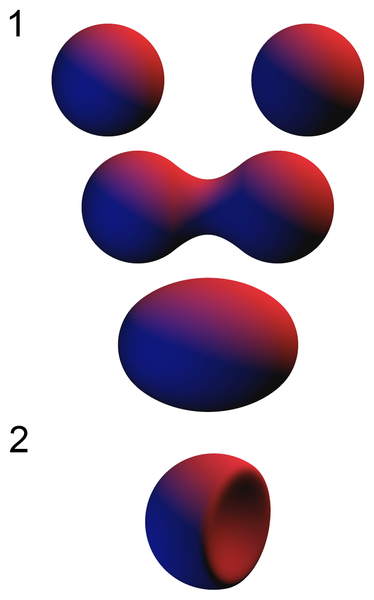
\includegraphics[width=0.3\textwidth]{img/metaballs-concept.png}
	    		\caption{A conceptual visualization of how metaballs work. 1 shows two metaballs gradually merging, and 2 shows the influence of a negative metaball on a positive metaball. \cite{wiki07}}
	    		\label{fig:metaballs-concept}
	    	\end{minipage}
	    \end{figure}

    \section{Theory}

        \subsection{Metaball isosurface model}
            A metaball is an isosurface in 3D space. 
            Define a function $f(x,y,z)$, which takes as input a set of coordinates in 3D space, and returns a floating point value that represents the influence of the function on that point.
            When we have such a function, we can sample it at even or random intervals to determine which points belong inside the surface and which belong outside it.
            This is simply a matter of comparing whether the influence at a point is greater than a fixed threshold or not.
            We can then use a number of different rendering techniques to create a presentation of this 3D surface, as we shall see in the next section.

            For now, let us look at the metaball surface model in particular. The most common isosurface function for the metaball model is inverse quadratic:

            $[f(x,y,z) = 1.0 / (x^2 + y^2 + z^2)]$

            This function describes a field where each ball has an influence point with quadratic falloff.
            For any point $\vec{p}$ in 3D, and for any ball's position $\vec{b}$, the influence of that ball on the point $\vec{p}$ will be proportional to $|\vec{p} - \vec{b}|^2$.
            This function is also used to model the strength of electrical fields in electromagnetic studies, which is why we choose to label it as the metaball potential field function.
            \cite{geiss00}

            If one were to draw the resulting field of a single metaball around the origin, it might look like figure 2, where the brightness of the color indicates the influence of the field at that point.
            
            A similar model for two metaballs, with their potential fields partially overlapping in different stages, is shown in figure 3.
            
            \begin{figure}[H]
            	\centering
            	\begin{minipage}[b]{0.2\textwidth}
            		\centering
            		
\includegraphics[width=\textwidth]{img/2d-potential.png}
            		\caption{A concept of the inverse square function in 2D}
		            \label{fig:2d-potential}
            	\end{minipage}
            \end{figure}
        
        	\begin{figure}[H]
        		\centering
            	\begin{minipage}[b]{0.4\textwidth}
            		
\includegraphics[width=\textwidth]{img/2d-potential-multi.png}
            		\caption{A concept of 2 metaballs in 2D. Every frame shows the two balls moving closer to each other.}
            		\label{fig:2d-potential-multi}
            	\end{minipage}
            \end{figure}

            As you can see, the area between the two balls becomes gradually lit up.
            The intersection between two potential fields becomes brighter as the two balls move closer, and at some point the center point between the balls will have a strength that is above our threshold. This effect will propagate outwards as the balls move closer, and we will use this later to make the balls appear as if they blob together in 3D.

        \subsection{Marching cubes}
			Marching cubes is a well-known algorithm for constructing a polygonal mesh of an isosurface form a given scalar field. It was first published in the 1987 SIGGRAPH by William E. Lorensen and Harvey E. Cline, and was highly adopted in medical visualization.
			
			This algorithm takes a scalar field as an input, and output a list of triangles representing the isosurface. It iterates through the scalar field and calculate all corresponding value for each neighboring vertices in a voxel. Then depending on whether the value of neighbor vertices fall in or out of the isolevel, a list of triangle are generated according to the configuration. Since there are 8 vertices in a voxel, there are a total of 256 configurations of polygon placement as shown in figure 4. By combining all triangles generated within the scalar field, we can obtain the approximated polygonal mesh as a whole. 
			
			\begin{figure}[H]
				\centering
				\begin{minipage}[b]{0.4\textwidth}
					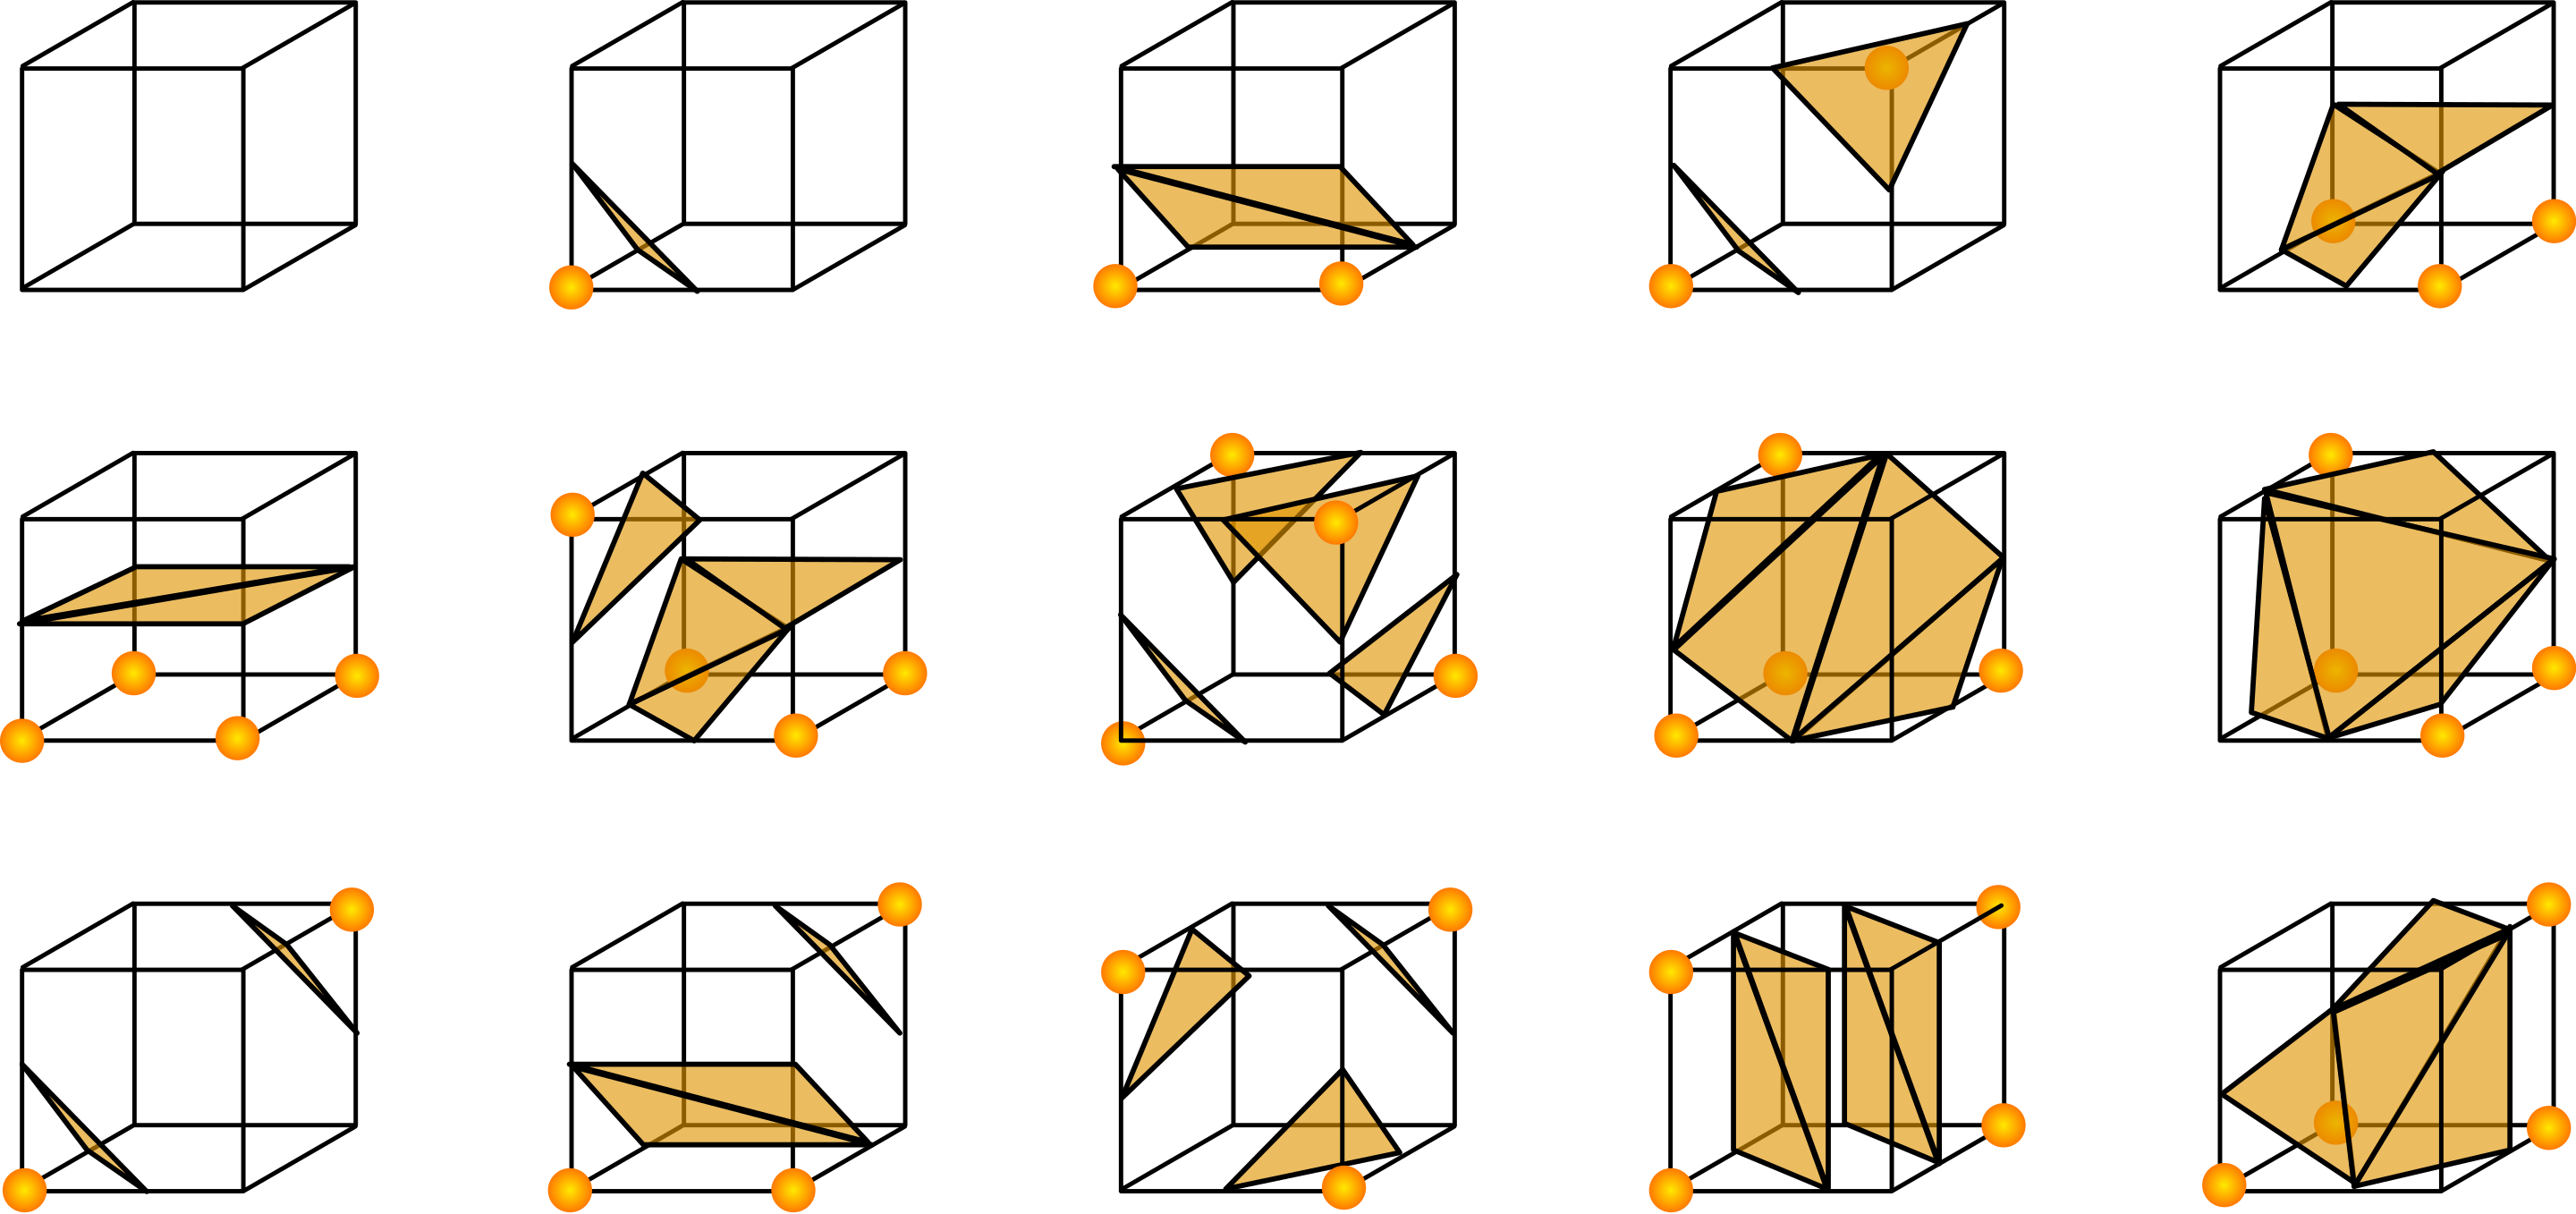
\includegraphics[width=\textwidth]{img/marching-cubes-config.png}
                    \caption{Marching cubes configurations \cite{wiki10}}
					\label{fig:marching-cubes-config}
				\end{minipage}
			\end{figure}
		
		\subsection{Smoothed Particle Hydrodynamics}
			Smoothed Particle Hydrodynamics (SPH) is a common computational method for simulating fluid flow on a machine. It was first published by Monaghan, Gingold and Lucy in 1977. In a SPH simulation, each fluid particle is interacting with its neighboring particle depending on its pressure, density, and velocity given a finite boundary around the particle. A particle's density is denoted as $$p_i=\sum_{j} m_jW_{ij}$$ where $W_{ij}$ can be any smoothing kernel. The pressure is then calculated with the ideal gas law in thermodynamics, written as $P=K(p-p_0)$. With the found density and pressure of a particle, we can find its acceleration by the following equation, $$a_i=-\sum_{j} \frac{m_j}{m_i}\frac{P_i+P_j}{2p_ip_j}\nabla W_{ij}\hat{r}_{ij}$$ where $\nabla W_{ij}$ is another smoothing kernel and $\hat{r}_{ij}$ is the normalized vector of a surrounding particle to the current particle. Finally, the particle position is being updated according to the computed acceleration. 

    \section{Implementation}

        We have used GLFW and GLSL. GLFW is a cross-platform utility library for creating window and OpenGL context, and we will use it for handling both window and input events. While GLFW handles all the high-level program logic, our project focuses on the low-level rendering. Mainly we will use GLFW to manage the OpenGL context. GLSL is the shading language for OpenGL which enables developers to control over the rendering pipeline. We will use GLSL to write our shader programs.
        
        The metaball positions are updated on the CPU, and sent to the GPU on every update frame. We encode the metaballs data as a $n\times1$ 2D Texture. Each pixel is encoded with the metaball position as its RGB values, and its radius as the alpha channel value. This method is proved ideal. Since Texture2D objects can be sent multiple times with different sizes, we can dynamically set the metaball count and the positions of each particles. Furthermore, since the Texture2D is easily sampled in a shader by using a Sampler object, it was trivial to extract the ball position and radius from each pixel.

        \subsection{Marching cubes}
        	We took the inspiration from Cyril Crassin's GLSL implementation. \cite{crassin} However, instead of representing the scalar field with 3D texture, we used a vertex buffer storing each voxel position in the grid. Also, we used a 2D texture for encoding the metaballs position and radius. The following pseudo-code is a brief description of our marching cube algorithm implementation in a geometry shader.
        	
			\begin{algorithm}[H]
				\KwIn{A voxel center position}
				\KwOut{A triangle list representing the isosurface}
				Corners[8] $\leftarrow$ Position of 8 voxel corners\;
				\For{$i\leftarrow 0$ \KwTo $7$}{
					\For{$j\leftarrow 0$ \KwTo $MetaballCount-1$}{
						Pixel $\leftarrow$ MetaballTex[0][j]\;
						IsoValue[i] $\leftarrow$ Pixel.a / distance(Pixel.rgb, Corners[i])\;
					}
				}
				LookUpIndex $\leftarrow$ 0;
				\For{$i\leftarrow 0$ \KwTo $7$}{
					\If{IsoValue[i] $<$ IsoLevel}{
						LookUpIndex $\leftarrow$ LookUpIndex + $2^i$\;
					}
				}
				\If{LookUpIndex = 0 $\vee$ LookUpIndex = 255}{
					return\;
				}
				VertexList[12] $\leftarrow$ Position where isosurface intersects 12 voxel edges\;
				\While{LookUpTex[LookUpIndex][i] != -1}{
					P1$\leftarrow$VertexList[LookUpTex[LookUpIndex][i]]\;
					P2$\leftarrow$VertexList[LookUpTex[LookUpIndex][i+1]]\;
					P3$\leftarrow$VertexList[LookUpTex[LookUpIndex][i+2]]\;
					Triangle $\leftarrow \bigtriangleup$(Pt1, Pt2, Pt3)\;
					Triangle.normal $\leftarrow$ cross(Pt3-Pt1, Pt2-Pt1)\;
					OutPrimitives.append(Triangle)\;
				}
				\caption{Marching Cubes}
			\end{algorithm}
        	
			This geometry shader code takes in a voxel position and outputs the sequence of polygonal mesh of the isosurface. We have two input textures, one for triangle configurations look-up ($LookUpTex$), and one for the encoded information for our metaballs ($MetaballTex$). 
			
			From line 1 to 5, the isovalue for each corner vertices is evaluated according to the inverse quadratic equation. With all the isovalue calculated, we then have to figure out which cube configuration should be used. And it can be done by comparing each vertex to the threshold ($IsoLevel$) and construct a bitmap $LookUpIndex$, as shown in line 6 to 8. In line 9 and 10, we terminate the algorithm since the voxel is considered as entirely inside or outside of the surface if $LookUpIndex$ is 0 or 255. That means no polygonal mesh is needed to be rendered. After that, every vertices along the voxel edges are interpolated based on the isovalue of the two neighboring corners. 
			
			With the correct configuration index and vertices position, we can construct the triangle list that is going to be rendered. Noted that every single row in the $LookUpTex$ follows this layout:
			\begin{minipage}{\linewidth}
				\begin{lstlisting}
				{2, 8, 3, 2, 10, 8, 10, 9, 8, -1, -1, -1, -1, -1, -1, -1}
				\end{lstlisting}
			\end{minipage}
			A row consists of 16 integers initialized with -1. Starting from the left, every three integers specify which three vertices along the edge make a triangle. There will be a maximum of 5 triangles in any cube configurations, leaving the last integer in the layout a padding space. From line 12 to 18, we query the suitable edge index from $LookUpTex$ and find its corresponding interpolated vertex position in $VertexList$ as the final triangle vertex position. Using the three vertices, we can calculated the face normal easily for later use in fragment shading stage. And finally push the triangle to the end of the output triangle stream. Repeat this process until there are no triangles needed to be added to the list. 
        
		\subsection{Smoothed Particles Hydrodynamics}
			We followed the simplified version of SPH from the paper written by Ryan L. Guy. \cite{guy15} Given the basic governing equations for modeling fluid flow, we are able to visualize a more fluid-like interactions between our metaballs. This physical simulation is evaluated on the CPU every frame. The final particle position is then mapped to our GPU shader for visualization purpose. Here is a pseudo-code describing how particles are simulated using SPH: 
			
			\begin{algorithm}[H]
				\KwData{$m := mass$, $P := pressure$, $p := density$, $a := acceleration$.}
				\ForEach{ball $\in$ Metaballs}{
					\ForEach{neighbor $\in Metaballs - \{ball\}$}{
						Dist $\leftarrow$ distance(ball, neighbor)\;
						$p_{ball} \leftarrow p_{ball} + m_{neighbor}\ *$ Poly6SmoothingKernel(Dist,$SmoothingRadius$);
					}
					$p_{ball} \leftarrow max$($p_{ball}$, $MinDensity$)\;
					$P_{ball} \leftarrow$ PressureConstant$ * $($p_{ball}$)\;
				}
				\ForEach{ball $\in$ Metaballs}{
					\ForEach{neighbor $\in Metaballs - \{ball\}$}{
						Dist $\leftarrow distance$(ball, neighbor)\;
						$\hat{r} \leftarrow normalize($ball.position - neighbor.position)\;
						$a_{ball} \leftarrow a_{ball} +  \frac{m_{neighbor}}{m_{ball}}\cdot\frac{P_{ball}+P_{neighbor}}{2\cdot p_{ball}\cdot p_{neighbor}} * \hat{r}\ * $ SpikyGradientKernel(Dist, $SmoothingRadius$)\;
					}
					$a_{ball} \leftarrow a_{ball} + Gravity$\;
				}
				\caption{SPH Simulation}
			\end{algorithm}
			
			We tested multiple configurations for our constant values, and we found that $SmoothingRadius = 0.1, PressureConstant = 20.0, MinDensity = 0.0$ is the most ideal value for presenting a realistic fluid.

			In order to find a particle's acceleration, we have to find out its density and pressure first. The first for-each loop is performing such calculation. We compare every pairs of particle, and sum up the neighboring particle's influence by multiplying neighbor's mass and applying a smoothing kernel. Here we use the poly6 smoothing kernel to filter out particles which is located outside its soft boundary: 
			
			\noindent
			\begin{minipage}{\linewidth}
				\begin{lstlisting}[escapeinside={(*}{*)}]
				//  (*$ \textcolor{dkgreen}{W_{ij}= 315*(h^2-r^2)^3 / 64*\pi*h^9} $*)
				float Poly6SmoothingKernel(float r, float h)
				{
				return (*$ 315 * (h^2 - r^2)^3 / 64 * \pi * h^9 $*);
				}
				\end{lstlisting}
			\end{minipage}
		
			The particle pressure is then calculated using ideal gas law in line 6. With the density and pressure found, we can proceed to calculate its acceleration. In the second for-each loop, each particle is once again compared to its neighboring particles. $\hat{r}$ is the normalized direction which the particle should travel under a repelling force. The acceleration is taken account with neighboring particles and the spiky gradient kernel. The spiky gradient kernel is defined as:
			
			\noindent
	        \begin{minipage}{\linewidth}
	        	\begin{lstlisting}[escapeinside={(*}{*)}]
	        	//  (*$ \textcolor{dkgreen}{\nabla W_{ij} = -45*(h-r)^2/\pi*h^6} $*)
	        	float SpikyGradientKernel(float r, float h)
	        	{
	        	return (*$ -45 * (h-r)^2 / \pi * h^6 $*);
	        	}
	        	\end{lstlisting}
	        \end{minipage}
        
        	Finally, the $Gravity$ which is set to be -9.8 towards the negative y-axis direction was added to the particle's acceleration in line 12. A fluid simulation cycle is now completed. This would keep repeating and updated in every single frame. 

        \subsection{Misc}
            For the purpose of creating a nice demo, we created a fragment shader with basic Phong illumination, in order to give the animation more depth.
            We also added a physics model to the balls which consists of outer forces due to gravity and a repelling force between each pair of balls when they are close to each other, to prevent them from accumulating in one place.
            We also modeled the bounciness of the floor and walls of our simulation domain, in order to keep the balls confined and in motion for as long as possible.

            We will not go into the details of how we implemented physics and the illumination model, as they are out of the focus of this report.

    \section{Result}
        Figure 4 shows three still images of our final rendering. 
        An animated video can be found here:
        \url{https://youtu.be/jmScNqchXs0}.

        Both the figure and the video show the same real time simulation, consisting of 100 particles and a voxel grid size of 80 units.
        The same physics and lightning models that were mentioned at the end of section 4 have both been applied.

        \begin{figure}[H]
        	\begin{minipage}[b]{0.5\textwidth}
	            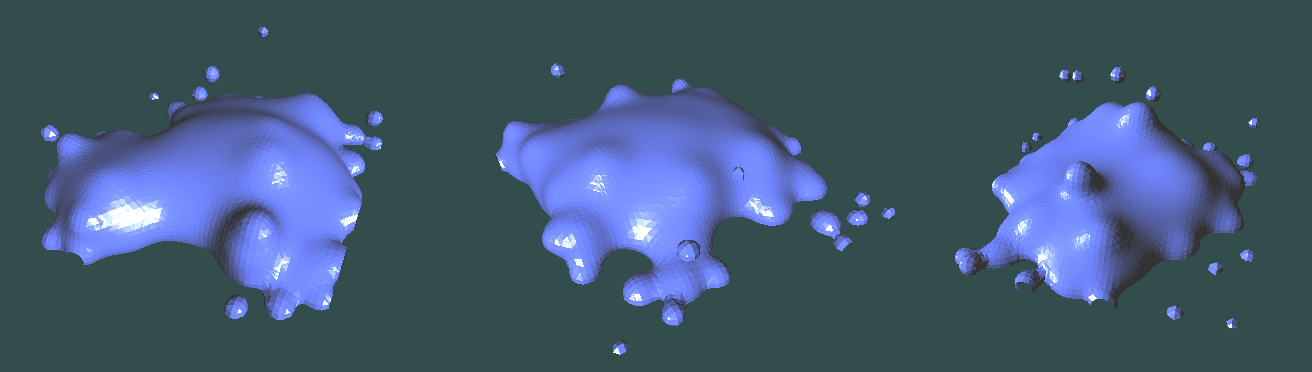
\includegraphics[width=\linewidth]{img/result-animation.png}
				\caption{Screenshot of the final animation, taken at fixed intervals. Note that the camera view is rotating around the model at a constant speed.}
				\label{fig:result-animation}
        	\end{minipage}
        \end{figure}

    \section{Conclusions}
    
        \subsection{Limitations on the rendering model}
        
        One of our main obstacles with the simulation was that we could not run it with a high enough voxel grid count to render an impressive looking fluid on a large simulation domain.
        The cell count of the voxel grid is simply the resolution at which the fluid can be rendered.
        A high enough cell count will make the fluid appear smooth and seamless, but as the cell count decreases, the sharp edges of the cube marched mesh will become visible and the mesh as a whole will appear coarse and chunky.

        In order to find out whether the voxel shader or the particle model were the performance bottleneck, we ran a series of tests of the same simulation, with varying numbers of particles.
        The test was run on a NVIDIA Geforce GTX 1050 Ti, which can be classified as a medium-tier to high-tier laptop graphics card.
        For each test we noted the maximum voxel cell count we could use while still running the simulation reliably above 30 frames per second.
        The following table lists the number of metaballs vs the maximum voxel grid cell count we could use before the frame rate would drop below 30 fps:

		\noindent
        \begin{tabular}{ c | c | c }
            voxel grid size & max balls at 30 fps & max balls at 60 fps \\
            80 & 180 & 130 \\
            50 & 295 & 205 \\
            20 & 295 & 205 \\
            5 & 300 & 210 \\
        \end{tabular}

        Finally: disabling the metaball filter completely, and just running the voxel shader itself, yielded a maximum voxel cell count of 310 units before the frame rate dropped below 30.
        Our conclusion is that the geometry shader itself, without any particles, can run with a voxel grid size in the order of 100-200 units at 60 fps, and up to 300 units at 30 fps.
        For our purpose, this can be used to create a nice looking dynamic fluid on a small simulation domain, or a very chunky looking fluid on a medium sized to large sized simulation domain, or a fluid with very few particles.
        To render an impressive fluid in a medium sized voxel grid, it would be nice if we could optimize the particle model so that we could run in the order of 100 particles at a voxel grid size of 200.
        The following section about the particle model will discuss some ideas for how this could be achieved in theory.

        \subsection{Particle model, optimizations to the SPH algorithm}
        It seems that the industry standard for fluid simulation in high quality games and video is the Smoothed Particle Hydrodynamics (SPH) model with Ellipsoid Splatting rendering.
        The SPH model uses nearest neighbor search to find out how a particle should collide.
        Ryan L. Guy, whose SPH implementation we created a naive version of, has profiled his simulation times in his paper for the University of Virginia. From the results we can see that the majority of the simulation time (around 75\%-85\%) is spent in the nearest neighbor search.
        Thus the goal for the particle model must be to optimize the nearest neighbor search for all particles.
        \cite{guy15}
        Guy has done this by implementing a spatial grid that functions as a lookup table for the particles, while our implementation uses a brute force search over all other particles.
        This severely limits the number of particles that can be modeled, 
        For each voxel grid cell, all particles and their influences on that point are taken into account, even if they are so far away that their contribution of the field is negligible.
        We can however use Guy's idea of spatial subdivision, by assigning the particles to their own grid cells, to determine which range of particles should realistically have influence over a given point, before iterating through them 
        Any particle will begin its nearest neighbor search in the grid cell in which it is contained, and continues to search through the nearest 26 cells until the nearest-neighbor is found.
        The fixed grid size was set to the one smoothing radius of the particle system, which is the maximum distance at which any two particles will interact.
        We imagine implementing this as a spatial structure that is embedded in the texture that sends the particle positions to the GPU.
        Each Y-coordinate of the texture could represent a grid cell, and all pixels on that column would still represent the particles that are in that cell, their positions and sizes.
        Even after transforming the 3D grid to a linear structure one could simply define a lookup function that continues the nearest neighbor search in the neighboring cells, and terminating after a certain depth if no neighbor particles are found.
        We could very well experiment with different values of the smoothing radius and thus the fixed grid size, but a good initial guess might be the radius from a particle center at which the potential field evaluates to some low threshold, let us say 0.01. 
        This form of spatial subdivision would allow for more particles in the simulation, but since the voxel shader itself cannot run reliably with a grid size above 200-300 units, it would not yield the necessary performance increase that is needed to simulate particles in a high-resolution domain.

        \subsection{Optimizations to the metaballs rendering technique}
        Yet another performance problem comes from the fact that the division step in our metaball potential function is computationally expensive.
        Ryan Geiss (whose tutorial on the metaball isosurface model we used for this project) came with a suggestion for an approximate polynomial function which should in theory be faster on the GPU. His suggested function was:

        \begin{center}
        $[g(r) = r^4 - r^2 + 0.25]$
        \end{center}

        This potential field function also has the neat property that it evaluates to 0 at $r=\frac{1}{\sqrt{2}}$, which means that you could do spatial optimization by only evaluating the points that fall within the radius of $r=\frac{1}{\sqrt{2}}$ of a singe metaball's center.
        \cite{geiss00}
        Our prediction is that this would yield a similar performance increase to implementing a naive spacial subdivision, but we are still not solving the problem that the voxel shader itself is expensive.
        To address this, our suggestion would be to redo the rendering model and instead use a point-based rendering method, which would be much more ideal for real time fluid simulation.

        \subsection{Summary}
        To conclude, we believe that the key to a more impressive fluid simulation is to optimize our SPH implementation so that each particle can do the nearest neighbor search more selectively, as well as to use another rendering method, other than the marching cubes method.
        We suggest looking at point splatting for this, which is simply a method of rendering a circle or ellipsoid at the particle's position, that orients itself depending on the surface direction.
        If many particles accumulate in one area, that area will appear to be more concentrated.
        Much in agreement with our hypothesis, it seems that this is a standard method when it comes to rendering fluids in real time.
        Since point-based methods operate on a boundless point cloud, they also has the nice property of being domain-independent, which means you don't need to confine the fluid to a bounding box as in the case of marching cubes or any other voxel-based rendering method. This would make them more ideal for use in a game environment.

    \section{Division of responsibility}

    Alexander created the backbone GLFW program that first allowed us to render simple triangles and primitive shapes. He also implemented the metaballs rendering model and the potential field solution, and wrote a basic physics model, that Tsz Kin later used in the SPH model.

    Tsz Kin programmed a voxel shader and turned it into the marching cubes shader that we finally used. Additionally he implemented Ryan Guy's SPH model that made the particles interact with each other and the environment.

    \section{Reflections on the project}

    By far, the biggest problem we encountered was a graphical glitch that only occured on one of our computers. Inside the shader program we had not initialized the vec3 array containing the metaball positions, meaning that upon declaration it was given whatever values were stored in memory before. This resulted in strange behaviors, and what made debugging hard was that our computers treated this error differently.
    When the program was compiled and run on Tsz Kin's MacBook Pro, the simulation seemed to work perfectly fine, whereas on Alexander's linux PC we encountered these glitches. This led us to believe that we were actually running different version of OpenGL, and we began debugging library compatibility issues. We only found out after explaining the problem to a teacher's assistant, but by then we had spent a week without making any progress.

    Needless to say, we have learnt our lesson of the importance of manual memory management.
    We only maintain that a lot of time could have been saved, had we thought of this before.
    After all there is no denying that the task was of a very hard level for someone of our knowledge level of C++. 

    Other than that we did not encounter a lot of problems, and the project as a whole has been a stimulating and fascinating journey.
    We belive it was a good project because the hierarchical nature of it, which allowed us to progress just as far as we wanted.
    We could easily begin with creating a simple Hello Triangle application, and we could keep building on that, always having the next intermediate goal in mind, all the way to the final render.
    Both of us appreciate the we now have the overall OpenGL knowledge required for graphics and games programming, and we will most likely use this very project as a base to start future work on.
    When debugging we also got to use renderdoc to examine our shader programs, which we both now have valuable experience with.
    Our computers treated this differently. When compiled and run on Tsz Kin's MacBook Pro, the simulation seemed to work perfectly fine, whereas on Alexander's Linux PC we encountered these glitches. This led us to believe that we were actually running different version of OpenGL, and we began debugging library compatibility issues. We only found out after explaining the problem to a teacher's assistant, but by then we had spend a week without making any progress.

    \section{Idea for a perceptual study}

        Our idea for a perceptual study concerns the perception of 3D fluids with different material properties, what feelings they invoke in an observer and how the observer relate them to known fluid materials in the real world. Such data can be of use for e.g. 3D filmmakers who use materials not only to give an object features that are representative of the real world, but also to invoke emotions in the viewer, such as feelings of happiness, ease or horror.

        \subsection{Hypothesis}

            We assume that we can model fluid objects with different colors, as well as different physical properties such as adhesion and viscosity, as well as material properties such as translucency and reflectiveness.
            Our question is then how variations in these properties will affect people's perception of the 3D scene.
            Our hypothesis is that a person would feel negative emotions when presented with a virtual fluid object that strongly resembles a fluid material that we are naturally repelled by, such as mucus, slime, sludge or urine, as compared to if they would see a virtual fluid that resembles something positive such as soft drink, cream or milk or simply water.

        \subsection{Target group}
        
            For us it would be interesting to compare the two segments: younger people who have consumed a lot of digital animation and video games, and an older segment who are not used to seeing 3D animation. We imagine the target ages of 10-20 years for the group who frequently consumes 3D media, and 60-80 years for the group that does not. Of course we would have an initial survey to verify their 3D media consumption habits.
            
        \subsection{Procedure}

            We would begin by making a simple fluid simulation with a scene model that can collide with a fluid object, e.g. the stanford bunny. In this scene, we will be able to cofigure the properties of the fluid and spawn a fluid body on top of the bunny model, so that the viscous and adhesive properties become clearly visible. For example, if the fluid is very adhesive, some particles of the fluid body would stick to the bunny. Our inspiration to this setup comes from a scene in the NVIDIA Flex demo, as seen in figure 6.
            \begin{figure}[H]
                \centering
                \begin{minipage}[b]{0.5\textwidth}
                    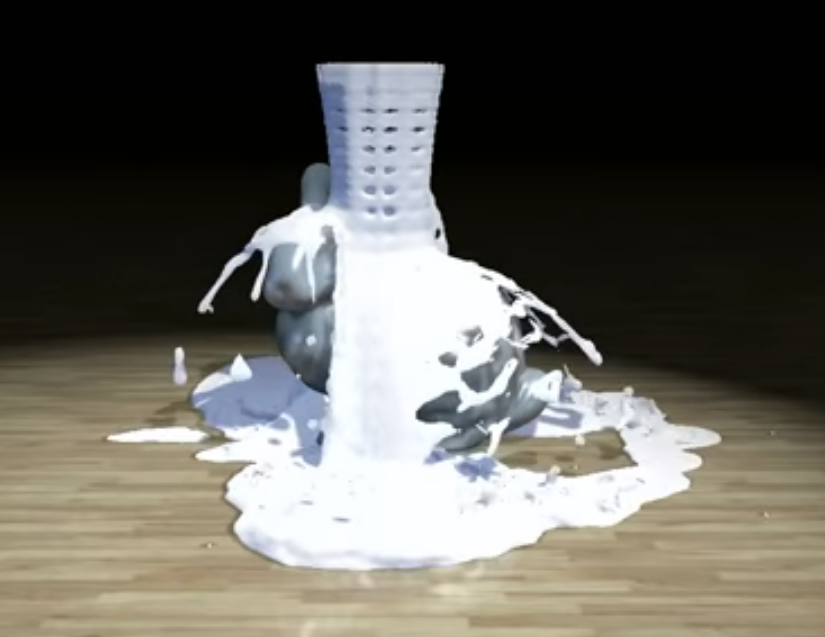
\includegraphics[width=\textwidth]{img/flex-bunny.png}
                    \caption{An example of how our scene could look, where a milk-like fluid interacts with a stanford bunny model. \cite{nvidia-flex}}
                    \label{fig:flex-bunny}
                \end{minipage}
            \end{figure}

            A few ideas for fluids we could model are:
            \begin{itemize}
                \item \textbf{Slime}: highly viscous, highly adhesive, green and very reflective but not very translucent.
                \item \textbf{Mucus}: not very viscous, highly adhesive, green/brownish and very translucent.
                \item \textbf{Milk}: not very viscous, not very adhesive, white and very reflective with no translucency.
            \end{itemize}

            We would show each respondent a random selection of fluids, perhaps 4 or 5, in a random order. The repondent then responds to a questionaire where we ask them questions about their experience with the animation. A few example metrics could be:
            \begin{itemize}
                \item How satisfied/dissatisfied the observer is.
                \item How pleased/disgusted the observer is.
            \end{itemize}
            
            Finally, we would ask the respondent what material they think the fluid represents, so that we can make a meaningful assesment of their answers based on what fluid they think they were percieveing. We would do this last of all, so as to not color the respondents' expectations when answering the other questions

        \subsection{Expectations}

            We have the predetermined notion that people are naturally disgusted by substances such as mucus and slime, so our expectation is that virtual representations of those fluids will invoke the same kind of emotion.
            Additionally, there is the possibility that failing to properly model a real fluid's visual or physical properties will cause a certain dissatisfaction in the observer. An example would be when a fluid that is known to be sticky, such as slime, does not stick to the scene model. We predict that the level of dissatisfaction would go up notably in these test cases.

	\end{multicols}

\begin{thebibliography}{9}

\bibitem{crassin}
	Cyril Crassin,
	\textit{OpenGL Geometry Shader Marching Cubes},
	January,
	2007.
	\\
	\url{http://www.icare3d.org/codes-and-projects/codes/opengl_geometry_shader_marching_cubes.html}

\bibitem{heckbert92}
	Paul Heckbert,
	\textit{Intro to Metaballs},
	November,
	1992.
	\\
	\url{https://steve.hollasch.net/cgindex/misc/metaballs.html}
	
\bibitem{geiss00}
	Ryan Geiss,
	\textit{Metaballs (also known as: Blobs)},
	October,
	2000.
	\\
	\url{http://www.geisswerks.com/ryan/BLOBS/blobs.html}

\bibitem{guy15}
	Ryan L. Guy,
	\textit{Smoothed Particle Hydrodynamics Fluid Simulation},
	2015.
	\\
	\url{http://rlguy.com/sphfluidsim/}

\bibitem{wiki07}
	Image from: \url{https://en.wikipedia.org/wiki/File:Metaballs.png}

\bibitem{wiki10}
  Image from: \url{https://en.wikipedia.org/wiki/File:MarchingCubes.svg}

\bibitem{nvidia-flex}
  Image from the official NVIDIA Flex demo video: \url{https://www.youtube.com/watch?v=1o0Nuq71gI4}

\end{thebibliography}

\end{document}
